\documentclass[xcolor={dvipsnames}]{beamer}

%%% PACKAGES %%%
\usepackage{graphicx}
\usepackage{tabularx}
\usepackage{booktabs}
\usepackage{multirow}
%\usepackage[usenames,dvipsnames]{color}
\usepackage{textpos}
\usepackage{tipa}
\usepackage{hyperref}
%\usepackage{pifont}

%\usepackage{caption}[2008/08/24]
%\usepackage{subcaption}

\usepackage{perpage}
\MakePerPage{footnote}

%%% TODOs %%%
\usepackage[dvipsnames]{xcolor}
\newcommand{\TODO}[1]{{\color{red}\textbf{[TODO #1]}}}

%%% FONT %%%
\usepackage{tgheros}

%%% BEAMER THEME %%%
\usetheme{default}
\usecolortheme{whale}
\usecolortheme{orchid}
\setbeamertemplate{navigation symbols}{} 
\setbeamertemplate{footline}[frame number]
%\setbeamertemplate{footline}{%
%  \leavevmode%
%  \hbox{%
%    \pgfsetfillopacity{0}\begin{beamercolorbox}[wd=.333333\paperwidth,ht=2.25ex,dp=1ex,center]{author in head/foot}%
%      \usebeamerfont{author in head/foot}\pgfsetfillopacity{1}\insertshortauthor
%    \end{beamercolorbox}%
%    \pgfsetfillopacity{0}\begin{beamercolorbox}[wd=.333333\paperwidth,ht=2.25ex,dp=1ex,center]{title in head/foot}%
%      \usebeamerfont{title in head/foot}\pgfsetfillopacity{1}\insertshorttitle
%    \end{beamercolorbox}%
%    \pgfsetfillopacity{0}\begin{beamercolorbox}[wd=.333333\paperwidth,ht=2.25ex,dp=1ex,right]{date in head/foot}%
%      \usebeamerfont{date in head/foot}\pgfsetfillopacity{1}\insertshortdate{}\hspace*{2em}
%      \insertframenumber{} / \inserttotalframenumber\hspace*{2ex}
%    \end{beamercolorbox}}%
%  \vskip0pt%
%}
\addtobeamertemplate{frametitle}{}{%
\begin{textblock*}{100mm}(.875\textwidth,-.9cm)

\includegraphics[height=.9cm]{uds-logo-text-white.png}
\end{textblock*}}
\setbeamertemplate{caption}{\insertcaption}
\setbeamerfont{caption}{size=\scriptsize}
\setbeamertemplate{itemize subitem}[circle]
%\setbeamertemplate{bibliography item}[text]
\setbeamertemplate{bibliography item}[triangle]
\setbeamertemplate{blocks}[rounded][shadow=true]


%%% COLORS %%%
\definecolor{MutedBlue}{RGB}{83,121,170}
\definecolor{UniBlue}{RGB}{0,71,116}
\definecolor{DarkPink}{RGB}{178,56,119}
\definecolor{LightPink}{RGB}{255,224,246}
\definecolor{LightBlue}{RGB}{214,255,255}

%\setbeamercolor{title}{fg=UniBlue}
%\setbeamercolor{frametitle}{fg=UniBlue}
\setbeamercolor{author in head/foot}{fg=UniBlue}
\setbeamercolor{title in head/foot}{fg=UniBlue}
\setbeamercolor{date in head/foot}{fg=UniBlue}
\setbeamercolor{page number in head/foot}{fg=UniBlue}
\setbeamercolor{normal text}{fg=darkgray}
\setbeamercolor{structure}{fg=UniBlue}
\setbeamercolor{itemize item}{fg=UniBlue}
\setbeamercolor{itemize subitem}{fg=UniBlue}
%\setbeamercolor{section in toc}{fg=MutedBlue}
%\setbeamercolor{subsection in toc}{fg=darkgray}
%\setbeamercolor{bibliography entry author}{fg=darkgray}
%\setbeamercolor{bibliography entry title}{fg=darkgray}
%\setbeamercolor{bibliography entry location}{fg=gray!80!black}
%\setbeamercolor{bibliography entry note}{fg=gray!90!black}
%\setbeamercolor{bibliography entry note}{fg=darkgray}
\setbeamercolor{block title}{bg=structure,fg=white}
%\setbeamercolor{block body}{bg={palette secondary}}


%%% BIBLIOGRAPHY %%%
\usepackage[%
	backend=bibtex,
	citestyle=authoryear,
	maxcitenames=2,
	maxbibnames=99,
	firstinits=true,
	url=false,
	doi=false,
	isbn=false, 
	%sorting=none,
	]{biblatex}
\addbibresource{../library.bib}
% to cite on the same slide use \footfullcite{jones00}
\renewcommand{\footnotesize}{\scriptsize}

%% TITLE PAGE INFO %%
\author[A. Vakil]{Anjana Sofia Vakil
%\\\texttt{[anjanav,apalmer]@coli.uni-saarland.de}
} 
\institute{
\includegraphics[height=4.5em]{uds-logo-text.png}\\Department of Computational Linguistics and Phonetics\\University of Saarland, Saarbr{\"u}cken, Germany}
\title{Automatic diagnosis and feedback for lexical~stress errors in non-native speech:\\
Towards a CAPT system for\\French learners of German}
%\subtitle{Investigating the impact of source language choice} 
\date[16.4.15]{Master's Thesis Colloquium\\16 April 2015}

%% DOCUMENT %%
\begin{document}
{
\setbeamertemplate{footline}{} 
\begin{frame}
  \titlepage
\end{frame}
}
\addtocounter{framenumber}{-1}





\begin{frame}{Lexical stress}
Some syllable(s) in a word more accentuated/prominent\footfullcite{Cutler2005}

\begin{center}
\begin{tabular}{ccc}
um$\cdot$FAHR$\cdot$en & vs. & UM$\cdot$fahr$\cdot$en \\
\textit{to run over} & & \textit{to drive around}\\
\end{tabular}
\end{center}

%\vspace{-1em}

\addtocounter{footnote}{-1}
\begin{itemize}
\item{German: variable stress placement, contrastive stress\footnotemark
%\footfullcite{Cutler2005}
}
\item{French: no word-level stress, final syllable lengthening\footfullcite{Michaux2013}}
\end{itemize}

\vfill

Goal: Computer-Assisted Pronunciation Training (CAPT) for lexical stress errors for French learners of German


\end{frame}

\begin{frame}
\frametitle{Outline}
\tableofcontents%[pausesections]
\end{frame}




\section{Motivation}
\begin{frame}{Motivation}
		\begin{figure}
			\centering
			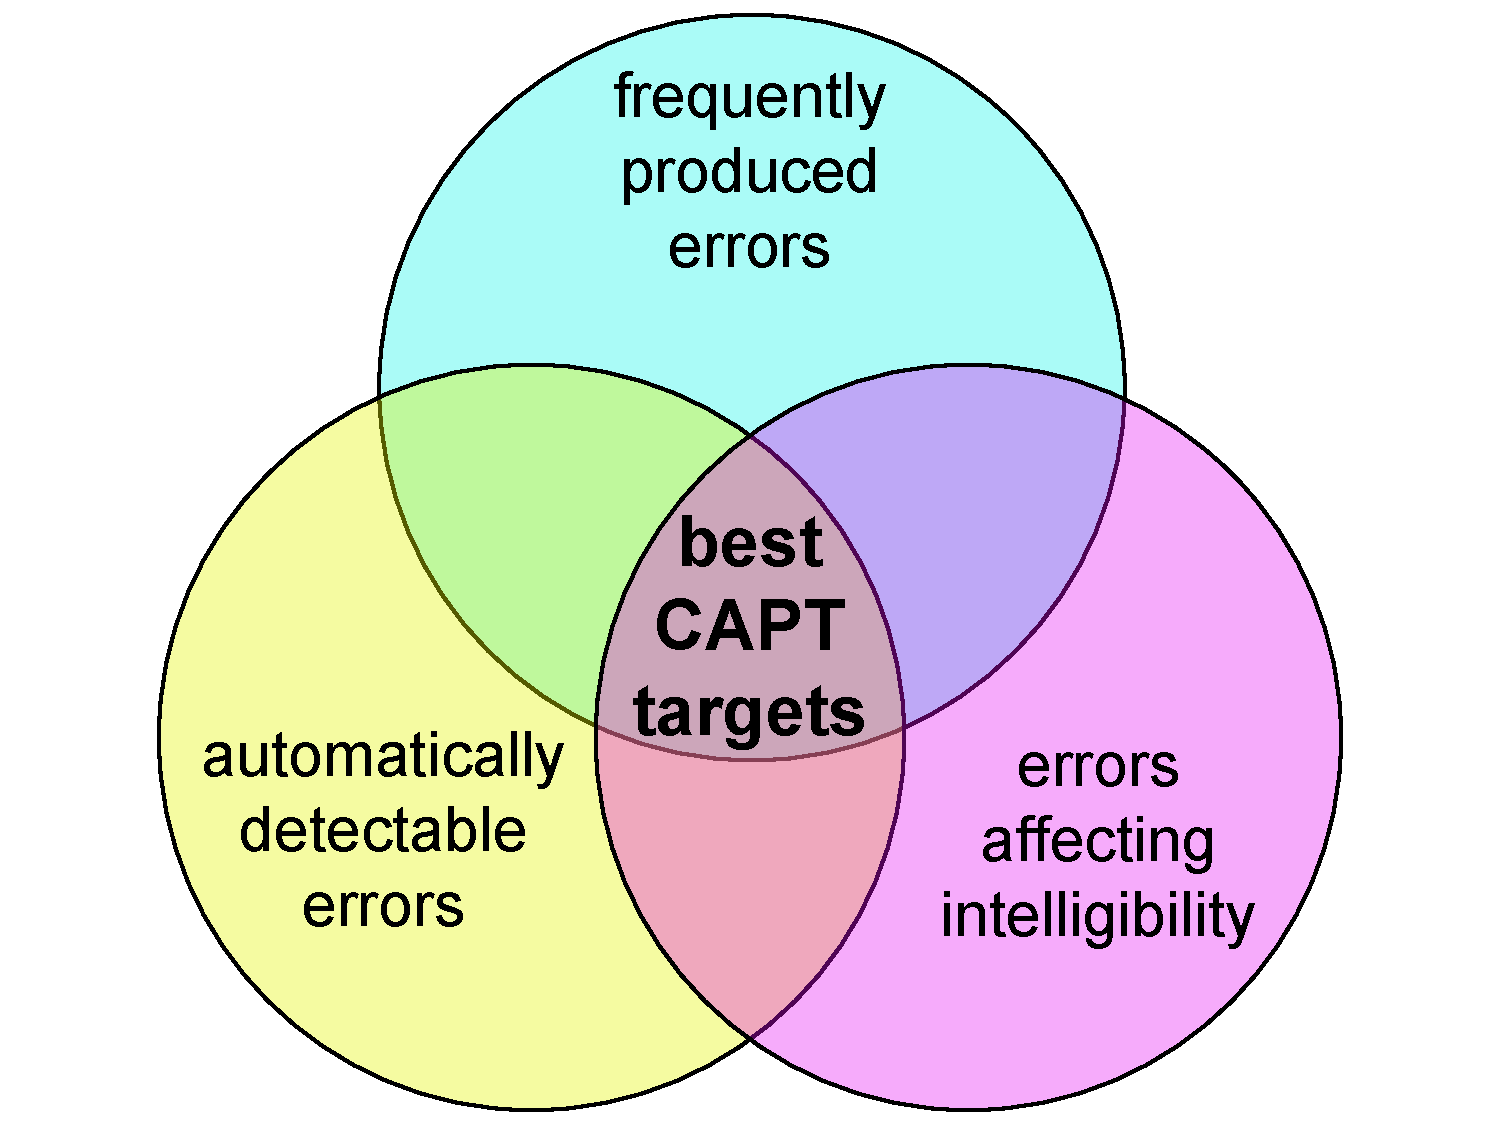
\includegraphics[width=.8\textwidth]{../img/error-venn}
			\caption{Criteria for selecting errors to target in a CAPT system.}
			\label{fig:errors}
		\end{figure}
\end{frame}

\begin{frame}{Motivation}
Lexical stress errors are: 
\begin{itemize}
\item Frequently produced by French learners of variable-stress languages\footfullcite{Bonneau2011}$^{,}$\footfullcite{Michaux2012}
\item More important for intelligibility in L2 German than other types of errors\footfullcite{Hirschfeld1994}
\item Possible to identify automatically by comparison$^1$ or classification\footfullcite{Kim2011}
\end{itemize}
\end{frame}

%\begin{frame}{Motivation}
%Frequently produced:
%\begin{itemize}
%\item French speakers perceptually ``deaf'' to Spanish stress\footfullcite{Dupoux1997}
%\item French learners make stress errors in Dutch\footfullcite{Michaux2012} and English\footfullcite{Bonneau2011}
%%\item French learners of Dutch (incorrectly) stress final syllables\footfullcite{Michaux2012}
%%\item French beginners frequently misplace English stress\footfullcite{Bonneau2011}
%\end{itemize}
%
%Affecting intelligibility:
%\begin{itemize}
%\item Prosodic errors impede intelligibility more than segmental errors
%\item Lexical stress errors have particularly strong impact on L2 German intelligibility\footfullcite{Hirschfeld1994}
%\end{itemize}
%
%
%Automatically detectable:
%
%\end{frame}

\section{Lexical stress errors by French learners of German}
	\subsection{Annotation of a learner speech corpus}
		\begin{frame}{\TODO{}}
		\TODO{}
		\end{frame}
	\subsection{Inter-annotator agreement}
		\begin{frame}{\TODO{}}
		\TODO{}
		\end{frame}	
	\subsection{Frequency of errors}
		\begin{frame}{\TODO{}}
		\TODO{}
		\end{frame}

\section{Error diagnosis}
	\subsection{Word prosody analysis}
		\begin{frame}{\TODO{}}
		\TODO{}
		\end{frame}		
	\subsection{Diagnosis by comparison}
		\begin{frame}{\TODO{}}
		\TODO{}
		\end{frame}
	\subsection{Diagnosis by classification}
		\begin{frame}{\TODO{}}
		\TODO{}
		\end{frame}

\section{Feedback}
	\subsection{Implicit}
		\begin{frame}{\TODO{}}
		\TODO{}
		\end{frame}
	\subsection{Explicit}
		\begin{frame}{\TODO{}}
		\TODO{}
		\end{frame}
	\subsection{Self-assessment}
		\begin{frame}{\TODO{}}
		\TODO{}
		\end{frame}

	
\section{The de-stress CAPT tool }
%	\subsection{For students}
%		\begin{frame}{\TODO{}}
%		\TODO{}
%		\end{frame}
%	\subsection{For teachers/researchers}
		\begin{frame}{\TODO{}}
		\TODO{}
		\end{frame}


\end{document}